\documentclass[journal,10pt,onecolumn,compsoc]{IEEEtran} \usepackage[margin=1.0in]{geometry} \usepackage{pdfpages} \usepackage{graphicx} 
\graphicspath{/graphics} \setlength{\parskip}{\baselineskip} \setlength\parindent{24pt}
\usepackage[english]{babel}
%\usepackage{fullpage}

\newcommand*\Title{WYSIWYG Approach to GUI for TensorFlow Deep Learning API}
\newcommand*\Date{October 2016}
\newcommand*\Author{Behnam Saeedi, Connor Sedwick, Collin Dorsett}
\newcommand*\GroupNumber{Group Number: 33}
\newcommand*\GroupName{Group Name: Visual Flow}
\title{WYSIWYG Approach to GUI for TensorFlow Deep Learning API}
\author{Behnam Saeedi, Connor Sedwick, Collin Dorsett}
\date{\today}

\begin{document}
\maketitle
\newpage
\tableofcontents
\newpage
\section{Introduction}

This section gives a scope description and overview of everything included in this SRS document. 
The purpose for this document is described and a list of abbreviations and definitions is provided within this section.

\subsection{Purpose}

The purpose of this document is to give a detailed description of the requirements for the WYSIWYG Deep Learning graphical user interface software. It will illustrate the purpose and complete declaration for the development of the system. It will also explain system constraints, interface and interactions with other external applications. 

\subsection{Scope}

The WYSIWYG Deep Learning graphical user interface is a desktop application which helps people design and test deep learning algorithms.
The application should be free to download and be usable on multiple operating systems.
Developers will be allowed to use their own data for input.
The software will be able to interface with Google's TensorFlow API. 

\subsection{Glossary}
\begin{itemize}
	\item Tensorflow:
		TensorFlow is an open source software library for numerical computation using data flow graphs.
		TensorFlow was originally developed by researchers and engineers working on the Google Brain Team within
		Google's Machine Intelligence research organization for the purposes of conducting machine learning and 
		deep neural networks research, but the system is general enough to be applicable in a wide variety of other domains as well.
	\item GUI:
		GUI or Graphical User Interface, Is an interface that allows users to interact with a given system through graphical icons and representation of tasks as oposed to a text base representation.
	\item Scene
		In our solution, Scene is the work space where user can place different elements of their program.
	\item Block:
		A block is a a GUI feature for the user to serve a specific purpose. A block could be variable/Constant, Method, class, probe input or output.
	\item Block-Menu:
		Block-Menu is a menu that contains all of the items and functionality icons that are ready to be dragged and dropped into the scene.
	\item Run
		In our solution, the task of starting executing the program is referred to as Running the program.
	\item Stop
		In our solution, stop brings the execution of the program to a halt. Resuming the process requires running the program again.
		This functionality will reset the state of the execution.
	\item Extract
		The task of creating the executable version of the program which is developed by our solution is referred to as extraction of the program.
		In order for a user to have a stand-alone version of their implemented program, they need to extract their project.
	\item Variable/Constant:
		Variables are equivalent to programming variables. They are represented by rhombus in our graphical user interface.
		Constants are similar to  variables, however, these values could not be changed while running the program.
		Constants are too represented by rhombus.
	\item Method:
		Methods are functions from the API that perform a specific task. They are represented by boxes.
		The circles on the edges of a method box are inputs and outputs of that method.
	\item Class: 
		In our solution, class refers to an object that contains multiple variables and methods (Public or private).
		Classes are represented as transparent boxes around methods and variables. This box could be abstracted away to be displays as a solid color box.
	\item Abstract:
		Abstract is feature of class that will turn the class from transparent to solid color in order to hide the content of the class.
	\item Layer: 
	\item Channel:
		 Channels are connections between inputs and outputs that display the direction of data flow and route the data from one block to another. 
	\item Probe:
		Probe is a UI element that displays the content of a channel.
		Probe can also modify the value which is being transmitted through the probe.
		If the value of a probe is modified, the modification will happen after the point which the probe is inserted into the channel.
		Every value that goes though the channel before the probe is left unchanged. (exception would be the pointer probes)
	\item input:
		Input is a UI element in our system which allows the user to insert data into their program during the run process.
	\item Output:
		Output is a UI element in our system which allows the user to see the final result. Outputs indicate discontinuation of a channel.
\end{itemize}
\subsection{References}
\subsection{Overview}

The remainder of this document includes three chapters. 
The second chapter provides an overview of the system functionality and system interaction with other libraries. 
Chapter two also introduces different types of stakeholders and their interaction with the system. 
Further, the chapter also mentions the system constraints and assumptions about the product.

The third chapter provides the requirements specification in detailed terms and a description of the different system interfaces. 
Different specification techniques are used in order to specify the requirements more precisely for different audiences.

The fourth chapter deals with the prioritization of the requirements. 
It includes a motivation for the chosen prioritization methods and discusses why other alternatives were not chosen.

\newpage

\section{Overall Description}

This section will give an overview of the whole system. 
The software will be explained in its context to show how the software interfaces with external libraries and introduce the basic functionality of it. 
It will also describe what type of stakeholders that will use the system and what functionality is available for each type. 
By the end, the constraints and assumptions for the system will be presented.

\subsection{Product Perspective}

The software will consist primarily of the graphical user interface which will communicate with Google's TensorFlow libraries. 
The software will need to have some way of ensuring that it has access to the TensorFlow libraries. 
The interface will provide to the user the basic design and flow of data through their program in a flowchart visual.
The underlying code and algorithm designed by the user will be stored in a file which is built and saved in the background. 

\subsection{Product Functions}

With the graphical user interface, users will be able to design an algorithm by placing uniquely shaped nodes in a build space and drawing connections between the nodes to represent dependencies and calls.
Build spaces represent either individual files, classes or layers. 
Files will be built based on the nodes and connections drawn between them in a build space.
These files can be extracted and saved to a user-designated folder at the push of a button.

Developers will be able to set probes on connections drawn between nodes to either modify values or track values as they are manipulated by their algorithm.
Helpful alerts will let the user or developer know if there is an error with the way they have designed their algorithm.

\subsection{User Characteristics}

There are many types of users who will likely use this software. 
As it stands, there is only one development layout to be used for the graphical user interface.
All users will be using the same desktop application whether they are students, developers, or employees whose project relies on deep learning software.

\subsection{Constraints}

This project is very user based and the only constraints are imposed on usability of our software and the core library that we are trying to mask.
The graphical user interface must be easily understood by the user and developer.
The display of results must be reliable and dependable.
The core system has its own limitations which will limit our GUI.

\subsection{Assumptions and Dependencies}

One assumption we have is that not all users will have prior knowledge on software programming when using this software.
A user may not know what a variable is or what a function is and how it relies on variables. 
When piecing together an algorithm a user may not know the proper syntax that would be required when using a text editing software.

A dependency for this software is access to Google's TensorFlow libraries from the user's memory space. 
This will require a user to install the libraries along with TensorFlow otherwise the software will not be usable in some scenarios.

\subsection{Apportioning of Requirements}

In the case that the project is delayed, there are some requirements that could be transferred to the next version of the application. 

\newpage

\section{Specific Requirements}

This section contains all of the functional and quality requirements of the WYSIWYG system. 
It provides a detailed description of the system and all its features.


\subsection{Interfaces}
\subsubsection{User Interfaces}

The graphical user interface will begin by displaying a menu allowing the user to "Start a new project."
Once this is chosen, the user will be brought to the main menu screen and build space.
From this screen the user will have the ability to choose different types of nodes for either coding or debugging purposes.
There will be buttons that allow users to build their file and run it.

Whenever a user wishes to pull the coded file of their algorithm in order to send it or apply it to other code they will have the ability to "Extract" the file.
This will be done by pressing a button and choosing a place in memory to store it. 
The file should be stored in the form of a .py file.

\subsubsection{Software Interfaces}

The graphical user interface should communicate with Google's TensorFlow API.
It should also communicate with the personal computer in the background to write the code file and executable file.
If an error message is thrown the interface should catch and display the error to the user as a formatted message within the GUI.

\subsection{Functional Requirements}

This section includes the requirements that specify the fundamental actions of the software system.

\noindent
\textbf{ID: FR1}\\
TITLE: Download the application\\
DESC: A user should be able to download the software from an application store or from GitHub. It should be free to download. 
The software should also come with a package of TensorFlow included.\\
RAT: In order for the user to download the software and have access to the require libraries.\\
DEPEND: None\\

\noindent
\textbf{ID: FR2}\\
TITLE: Open the GUI and start session\\
DESC: A user should be able to start a new session. \\
RAT: In order for the user to open up and start a new project with a blank build space.\\
DEPEND: FR1\\

\noindent
\textbf{ID: FR3}\\
TITLE: Session/Project Directory\\
DESC: The software should create a directory with a name specified by the user upon starting a new session or project.\\
RAT: In order for the software to build and store user files related to the current project in a main directory.\\
DEPEND: FR2\\

\noindent
\textbf{ID: FR4}\\
TITLE: Node Menu\\
DESC: The software should contain a node menu.\\
RAT: In order for the user to find nodes for the building of their algorithm.\\
DEPEND: FR2\\

\noindent
\textbf{ID: FR5}\\
TITLE: Build Space / Scene\\
DESC: The software should offer a blank space ox within the GUI for users to place nodes..\\
RAT: In order for the user to find nodes for the building of their algorithm.\\
DEPEND: FR2\\

\noindent
\textbf{ID: FR6}\\
TITLE: Drag and drop\\
DESC: The software should allow the user to drag nodes from the node menu and place them in a build space.\\
RAT: In order for the user to manipulate their algorithm.\\
DEPEND: FR3\\

\noindent
\textbf{ID: FR7}\\
TITLE: Channel drawing\\
DESC: The software should allow users to draw a channel between two nodes. 
This should be done simply by selecting them by clicking on them and choosing an option to "Draw channel".\\
RAT: In order for the user to send values between nodes.\\
DEPEND: FR3, FR4\\

\noindent
\textbf{ID: FR8}\\
TITLE: Node manipulation\\
DESC: The software should allow users to enter numerical and string values into variable nodes and probes.\\
RAT: In order for the user to write their algorithm.\\
DEPEND: FR4\\

\noindent
\textbf{ID: FR9}\\
TITLE: Background file creation\\
DESC: The software should create and update user-named files in the background as nodes are added to the build space. 
Files should be updated in a user-defined directory.\\
RAT: In order for the user to have a raw and formatted file of their software.\\
DEPEND: FR2, FR3, FR6, FR7, FR8\\

\noindent
\textbf{ID: FR10}\\
TITLE: Build button\\
DESC: The software should compile all files in the user's build directory at the single press of the build button. 
An executable file should appear in the user's current project directory if the algorithm compiles correctly.\\
RAT: In order for the user to create an executable in order to run the software.\\
DEPEND: FR4\\

\noindent
\textbf{ID: FR11}\\
TITLE: Error handling\\
DESC: The software should display a text box or error message to the screen letting the user know if there is an error with their build. 
There should also be a helpful hint on what the user may do to fix their problem.\\
RAT: In order for the user to know that there is an issue with the format of their current build of their software.\\
DEPEND: FR10\\

\noindent
\textbf{ID: FR12}\\
TITLE: Data input\\
DESC: The software should allow the user to include a file of their own data to be used by their software.\\
RAT: In order for the user to test their software on their own data.\\
DEPEND: FR2\\

\noindent
\textbf{ID: FR13}\\
TITLE: Layered builds\\
DESC: A user should be able to create multiple layers to their software by opening multiple build spaces.\\
RAT: In order for the user to visualize the structure of their software.\\
DEPEND: FR2\\

\noindent
\textbf{ID: FR14}\\
TITLE: File extraction\\
DESC: The software should allow the user to save their current build file to a user-defined space in memory.\\
RAT: In order for the user to have a raw and formatted file of their software in designated storage.\\
DEPEND: FR4\\


\subsection{Performance Requirements}

The requirements in this section provide a detailed specification of the user interaction with the software and measurements placed on the system's performance.

\noindent
\textbf{ID: QR1}\\
TITLE: Easy installation\\
DESC: There should be a simple downloadable package including everything required to begin using the software after installation.
There should be a different installation package depending on the operating system being used.\\
RAT: In order for the user to being using the software without having to worry about file dependencies.\\
DEPEND: None\\

\noindent
\textbf{ID: QR2}\\
TITLE: Prominent node menu\\
DESC: The node menu for the flowchart pieces should contain labelled nodes and be legible.\\
RAT: In order for the user to navigate the menu and find nodes easily.\\
DEPEND: None\\

\noindent
\textbf{ID: QR3}\\
TITLE: Prominent feature buttons\\
DESC: The buttons used to build and run the software should be easy to distinguish between each other. 
The extraction button should be indicated by as a button labelled "Extract".
Buttons should respond to a single click and respond within less than a second of the user clicking them.\\
RAT: In order to avoid confusion when trying to build and run the program.\\
DEPEND: None\\

\noindent
\textbf{ID: QR4}\\
TITLE: Prominent alerts\\
DESC: Alerts signaled by the compiler should be displayed to the screen as soon as they are sent. 
When an error has been fixed its corresponding alert should disappear.
Alerts should appear in colored text boxes: red boxes for fatal errors, yellow boxes for warnings.\\
RAT: This will cut down on confusion when rebuilding a file and trying to find issues with a solution.\\
DEPEND: None\\

\noindent
\textbf{ID: QR5}\\
TAG: Response time\\
DESC: The speed at which the interface communicates with the TensorFlow libraries and displays output to the screen.\\
SCALE: The time of a build.\\
METER: Measurements obtained by 1000 builds during testing.\\
MUST: No more than 3 seconds 100\% of the time.\\
WISH: No more than 2 seconds 100\% of the time.\\

%\subsection{Design Requirements}
%\subsection{Software System Attributes}
\newpage


\newpage
\section{References}
\newpage

\section{Gantt}
%\begin{figure}
	\begin{minipage}{\textwidth}
		\fbox{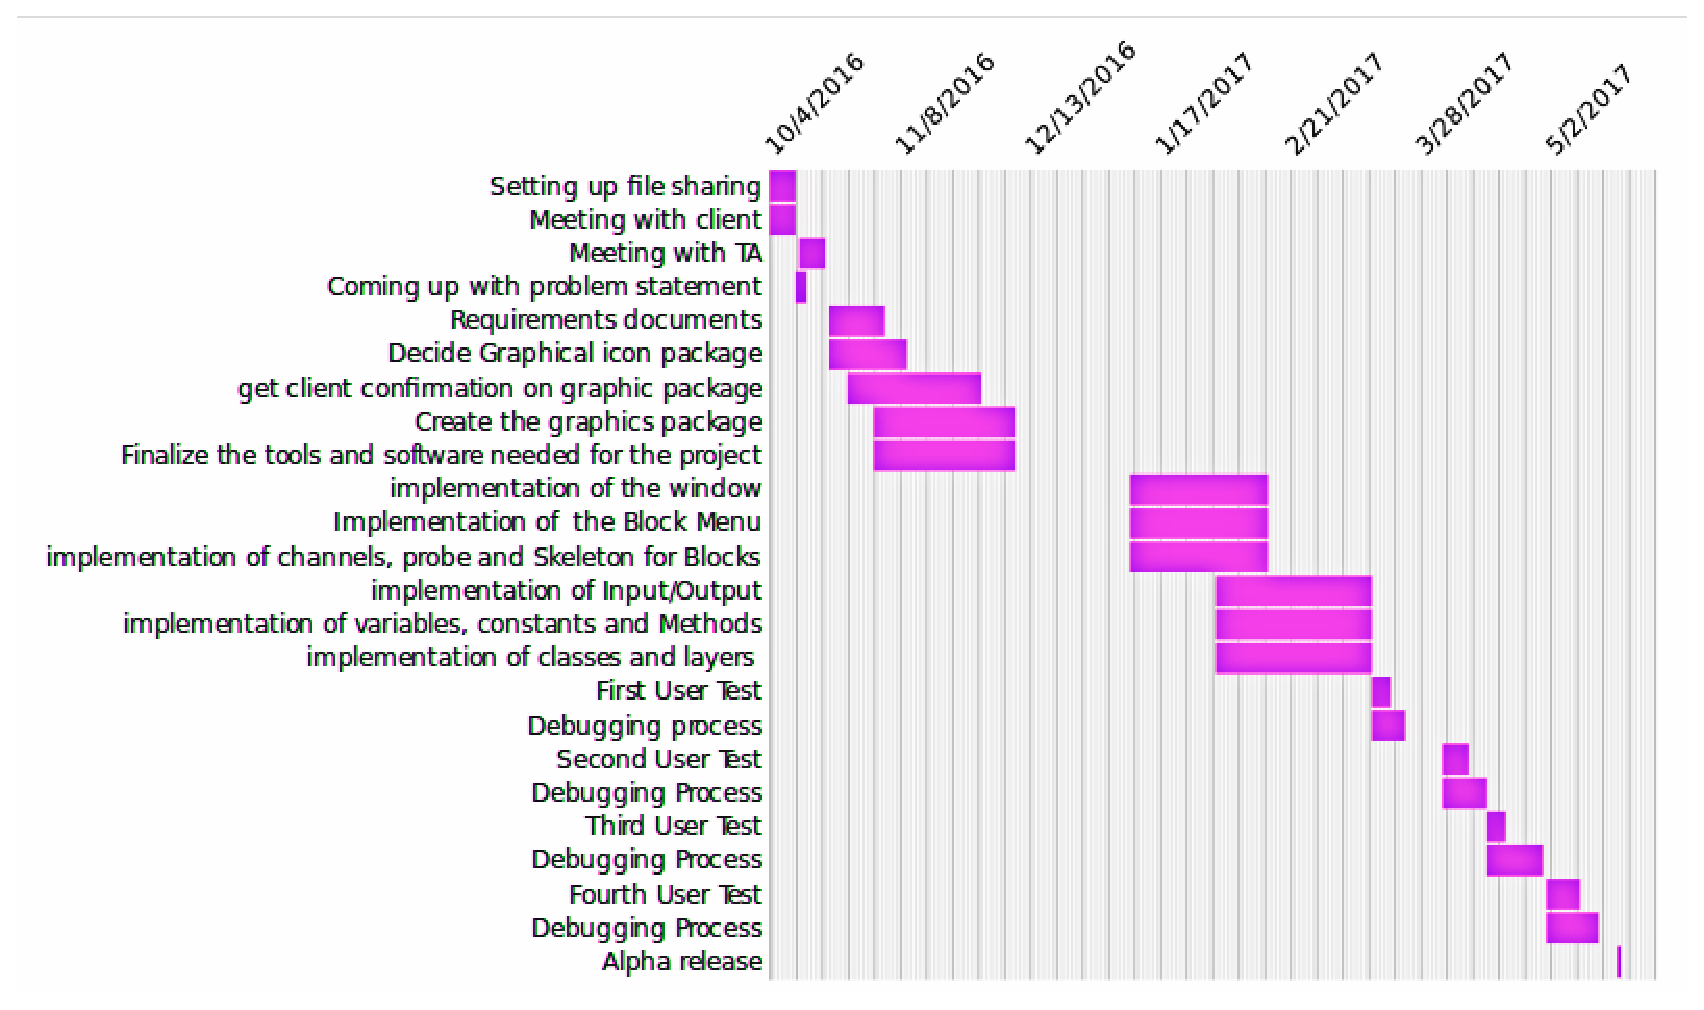
\includegraphics[width=1.0\textwidth]{graphics/Gantt-Chart.eps}}\\
%		\label{fig:fig1}
%		\caption{A proposed layout of the menu and build space.}
	\end{minipage}
%	\end{figure}

\end{document}
